\documentclass[11pt,a4paper]{article}
\usepackage[spanish]{babel}					% Utilizar español
\usepackage[utf8]{inputenc}					% Caracteres UTF-8
\usepackage{graphicx}						% Imagenes
\usepackage[hidelinks]{hyperref}			% Poner enlaces sin marcarlos en rojo
\usepackage{fancyhdr}						% Modificar encabezados y pies de pagina
\usepackage{float}							% Insertar figuras
\usepackage[textwidth=390pt]{geometry}		% Anchura de la pagina
\usepackage[nottoc]{tocbibind}				% Referencias (no incluir num pagina indice en Indice)
\usepackage{sectsty}						% Secciones sin enumeración
\usepackage{enumitem}						% Enumeraciones
\usepackage{mathtools}
\usepackage{amsmath}
\usepackage{amssymb}

\newcommand{\sign}{\text{sign}}

% Configuracion de encabezados y pies de pagina
\pagestyle{fancy}
\lhead{Vladislav Nikolov Vasilev}
\rhead{Aprendizaje Automático}
\lfoot{Grado en Ingeniería Informática}
\cfoot{}
\rfoot{\thepage}
\renewcommand{\headrulewidth}{0.4pt}		% Linea cabeza de pagina
\renewcommand{\footrulewidth}{0.4pt}		% Linea pie de pagina

\begin{document}
\pagenumbering{gobble}

% Pagina de titulo
\begin{titlepage}

\begin{minipage}{\textwidth}

\centering

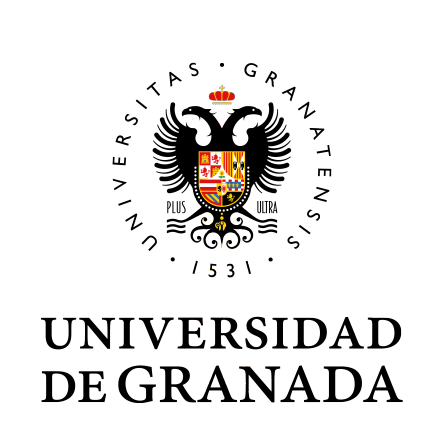
\includegraphics[scale=0.5]{img/ugr.png}\\

\textsc{\Large Aprendizaje Automático\\[0.2cm]}
\textsc{GRADO EN INGENIERÍA INFORMÁTICA}\\[1cm]

\noindent\rule[-1ex]{\textwidth}{1pt}\\[1.5ex]
\textsc{{\Huge MEMORIA PRÁCTICA 1\\}}
\noindent\rule[-1ex]{\textwidth}{2pt}\\[3.5ex]

\end{minipage}

\vspace{1.5cm}

\begin{minipage}{\textwidth}

\centering

\textbf{Autor}\\ {Vladislav Nikolov Vasilev}\\[2.5ex]
\textbf{Rama}\\ {Computación y Sistemas Inteligentes}\\[2.5ex]
\vspace{0.3cm}


\includegraphics[scale=0.3]{img/etsiit.jpeg}

\vspace{0.7cm}
\textsc{Escuela Técnica Superior de Ingenierías Informática y de Telecomunicación}\\
\vspace{1cm}
\textsc{Curso 2018-2019}
\end{minipage}
\end{titlepage}

\pagenumbering{arabic}
\tableofcontents
\thispagestyle{empty}				% No usar estilo en la pagina de indice

\newpage

\section{Ejercicio sobre la búsqueda iterativa de óptimos}

\subsection*{Apartado 1}
\noindent Implementar el algoritmo de gradiente descendente.\\

A continuación se muestra el código en Python implementado:

\begin{figure}[H]
\centering
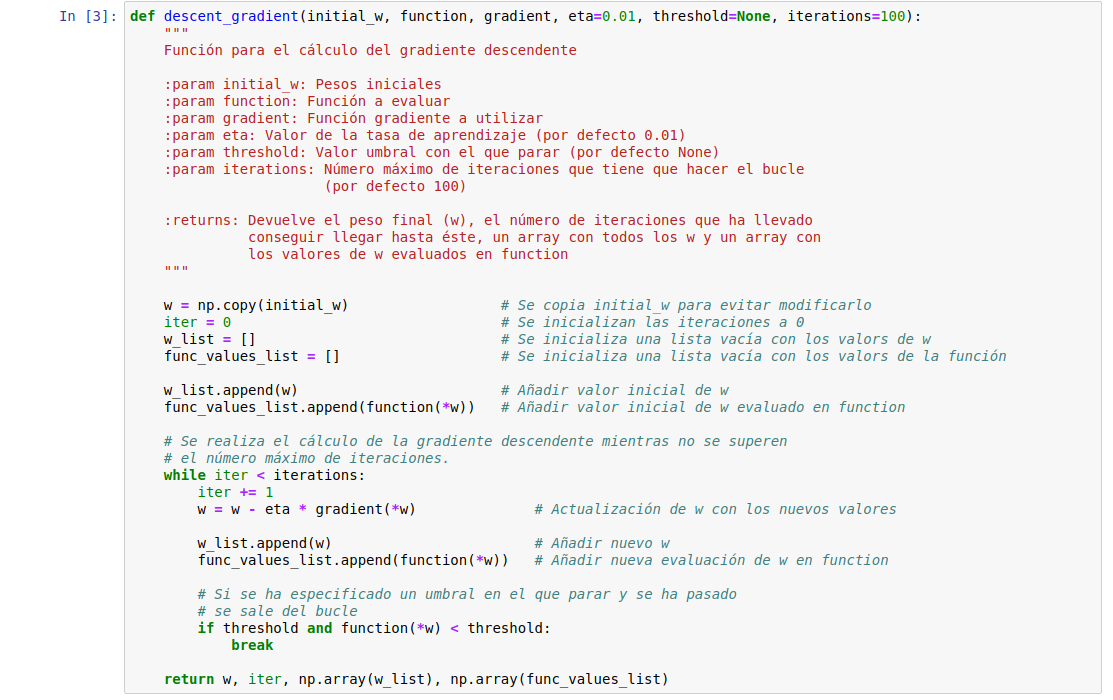
\includegraphics[scale=0.4]{img/descent_gradient_implementation.png}
\end{figure}


Se ha intentado que esta implementación sea lo más general posible para poder utilizarla en los ejercicios
posteriores, parametrizando la función que recibe (parámetro \textbf{function}), la cuál puede ser tanto
$f(x, y)$ como $E(u, v)$. Con este motivo, también se ha parametrizado el error con el que se quiere ajustar,
ya que en un caso no será necesario utilizar un error como criterio de parada (de ahí que su valor por defecto
sea \textbf{None}). Y, adicionalmente, se ha parametrizado el gradiente (parámetro \textbf{gradient}), para que
también se pueda especificar a la hora de la llamada cuál se usará. \\

\subsection*{Apartado 2}
\noindent Considerar la función $E(u, v) = (u^2 e^v - 2 v^2 e^{-u})^2$. Usar gradiente descendente para encontrar un
mínimo de esta funcón, comenzando desde el punto $(u, v) = (1, 1)$ y usanto una tasa de aprendizaje $\eta = 0.01$.

\begin{enumerate}[label=\alph*)]
	\item Calcular analíticamente y mostrar la expresión del gradiente de la función $E(u, v)$.
\end{enumerate}

Para calcular el gradiente, vamos a calcular antes $\frac{\partial E}{\partial u}$ y $\frac{\partial E}{\partial v}$.
Las derivadas, al aplicar la regla de la cadena, quedarían de la siguiente forma:

\begin{equation}
\begin{split}
\frac{\partial E}{\partial u}&= \frac{\partial}{\partial u} \Big( (u^2 e^v - 2 v^2 e^{-u})^2 \Big) = 2(u^2 e^v - 2 v^2 e^{-u})
\frac{\partial (u^2 e^v - 2 v^2 e^{-u})}{\partial u} = \\
 &=  2(u^2 e^v - 2 v^2 e^{-u})(2ue^v + 2 v^2 e^{-u})
\end{split}
\end{equation}

\begin{equation}
\begin{split}
\frac{\partial E}{\partial v}&= \frac{\partial}{\partial v} \Big( (u^2 e^v - 2 v^2 e^{-u})^2 \Big) = 2(u^2 e^v - 2 v^2 e^{-u})
\frac{\partial (u^2 e^v - 2 v^2 e^{-u})}{\partial v} = \\
 &=  2(u^2 e^v - 2 v^2 e^{-u})(u^2 e^v -4 v e^{-u})
\end{split}
\end{equation}

Con esto, tenemos que la expresión del gradiente es la siguiente:

\begin{equation}
\nabla E =
\left[
{
\begin{array}{c}
	\frac{\partial E}{\partial u} \\
	\\
	\frac{\partial E}{\partial v}
\end{array}
}
\right]
\end{equation}

\begin{equation}
\nabla E =
\left[
{
\begin{array}{c}
	2(u^2 e^v - 2 v^2 e^{-u})(2ue^v + 2 v^2 e^{-u}) \\
	\\
	2(u^2 e^v - 2 v^2 e^{-u})(u^2 e^v -4 v e^{-u})
\end{array}
}
\right]
\end{equation}

\begin{enumerate}[resume, label=\alph*)]
	\item ¿Cuántas iteraciones tarda el algoritmo en obtener por primera vez un valor de $E(u, v)$ inferior a $10^{-14}$?
	(Usar flotantes de 64 bits)
\end{enumerate}

\begin{figure}[H]
\centering
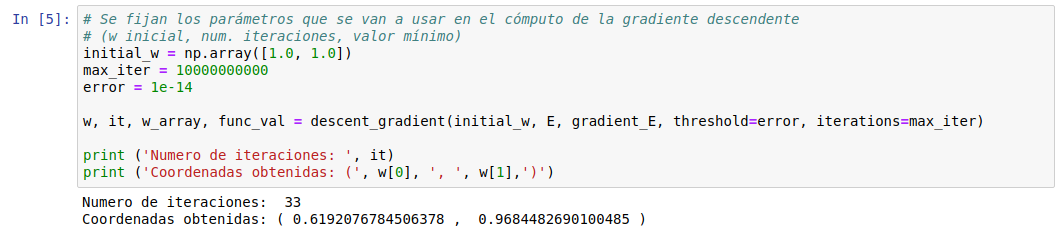
\includegraphics[scale=0.4]{img/jnbook_ej_2.png}
\caption{Cálculo del mínimo mediante el Gradiente Descendente para la función $E(u, v)$.}
\end{figure}

Como se puede ver en la figura anterior, donde también se incluye el código, el algoritmo tarda 33 iteraciones en encontrar
por primera vez un valor de $E(u, v)$ inferior a $10^{-14}$.

\begin{enumerate}[resume, label=\alph*)]
	\item ¿En qué coordenadas $(u, v)$ se alcanzó por primera vez un valor igual o menor a $10^{-14}$ en el apartado anterior?
\end{enumerate}

Las coordenadas donde se alcanzó un valor inferior a $10^{-14}$ son $(0.619, 0.968)$ (redondeadas a 3 cifras decimales).

\subsection*{Apartado 3}
\noindent Considerar ahora la función $f(x, y) = x^2 + 2y^2 + 2\sin(2 \pi x)\sin(2 \pi y)$.

\begin{enumerate}[label=\alph*)]
	\item Usar gradiente descendente para minimizar esta función. Usar como punto inicial $(x_0 = 0.1, y_0 = 0.1)$,
	tasa de aprendizaje $\eta = 0.01$ y un máximo de 50 iteraciones. Repetir el experimento pero usando $\eta = 0.1$,
	comentar las diferencias y su dependencia de $\eta$.
\end{enumerate}

Antes de mostrar las gráficas, vamos a calcular el gradiente de la función $f(x, y)$. Primero, vamos a calcular 
$\frac{\partial f}{\partial x}$ y $\frac{\partial f}{\partial y}$:

\begin{equation}
\frac{\partial f}{\partial x} = \frac{\partial}{\partial x} \Big(x^2 + 2y^2 + 2\sin(2 \pi x)\sin(2 \pi y)\Big) =
2x + 4 \pi \cos(2 \pi x)\sin(2 \pi y)
\end{equation}

\begin{equation}
\frac{\partial f}{\partial y} = \frac{\partial}{\partial y} \Big(x^2 + 2y^2 + 2\sin(2 \pi x)\sin(2 \pi y)\Big) =
4y + 4 \pi \sin(2 \pi x)\cos(2 \pi  y)
\end{equation}

\begin{equation}
\nabla f =
\left[
{
\begin{array}{c}
	\frac{\partial f}{\partial x} \\
	\\
	\frac{\partial f}{\partial y}
\end{array}
}
\right]
\end{equation}

\begin{equation}
\nabla f =
\left[
{
\begin{array}{c}
	2x + 4 \pi \cos(2 \pi x)\sin(2 \pi y) \\
	\\
	4y + 4 \pi \sin(2 \pi x)\cos(2 \pi  y)
\end{array}
}
\right]
\end{equation} \\

Una vez calculada la expresión del gradiente, vamos a ejecutar el código y a realizar la comparación de los cálculos 
del gradiente al cambiar el valor de $\eta$:

\begin{figure}[H]
\centering
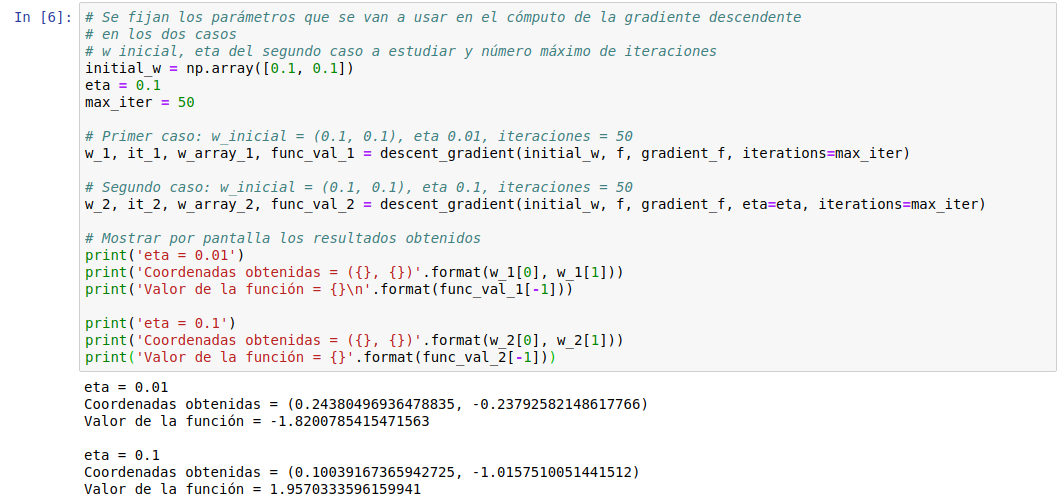
\includegraphics[scale=0.4]{img/jnbook_ej_3_a.png}
\caption{Valores de los óptimos para la función $f(x, y)$ cambiando $\eta$-}
\end{figure}

A continuación, se muestra el gráfico comparativo:

\begin{figure}[H]
\centering
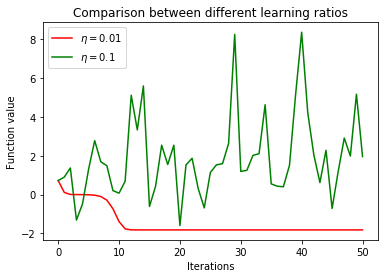
\includegraphics[scale=0.8]{img/comparison_lr.png}
\caption{Comparativa gráfica de la Gradiente Descendente con diferentes valores de $\eta$.}
\end{figure}

Como se puede ver, después de 50 iteraciones, al utilizar un $\eta = 0.01$ se consigue converger a un óptimo local, mientras
que al utilizar un $\eta = 0.1$ no se consigue. En el primer caso, los valores de $w$ van modificándose poco a poco con cada
iteración, y por eso en el gráfico que puede ver que tiene una forma muy suavizada el cambio que sufre $w$ entre iteración e
iteración. En cambio, en el segundo caso, al tener un $\eta$ mayor, se le da mucho peso al gradiente, y por tanto, los
valores de $w$ van modificándose muy bruscamente, como si estuviese oscilando entre la parte previa al mínimo y la
posterior, sin llegar a converger en ningún momento.\\

Por tanto, el valor de $\eta$ juega un factor clave en el algoritmo del descenso de gradiente. Si es muy bajo, los valores
de $w$ van descendiendo poco a poco, pero si el número de iteraciones son suficientes, se asegura llegar a un óptimo local.
Sin embargo, si el $\eta$ es muy grande, no se asegura en ningún momento que se pueda llegar al óptimo local, ya que puede
ir saltando entre la parte anterior y la posterior al mínimo indefinidamente, llegando incluso a poder alejarse de éste.

\begin{enumerate}[resume, label=\alph*)]
	\item Obtener el valor mínimo y los valores de las variables $(x, y)$ en donde se alcanzan cuando el punto de inicio
	se fija: $(0.1, 0.1), (1, 1), (-0.5, -0.5), (-1, -1)$. Generar una tabla con los valores obtenidos.
\end{enumerate}

A continuación se muestra una captura de pantalla con el código que permite generar los datos y la salida en formato tabla,
donde se muestran los 4 puntos con sus coordenadas iniciales, finales y valor del punto final.

\begin{figure}[H]
\centering
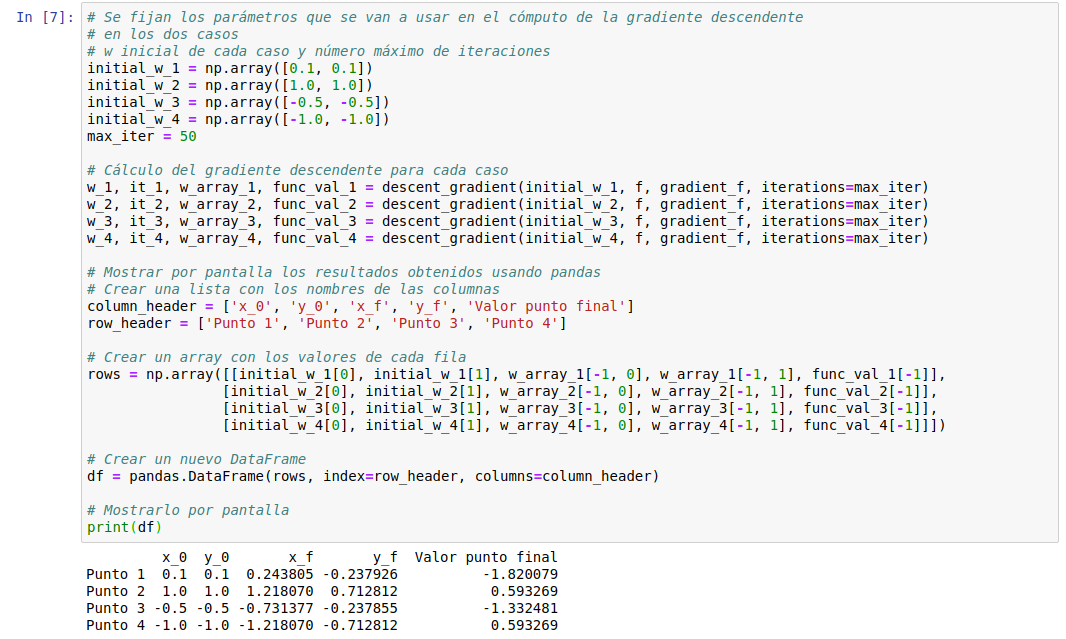
\includegraphics[scale=0.4]{img/jbook_ej_3_b.png}
\end{figure}

\subsection*{Apartado 4}
\noindent ¿Cuál sería su conclusión sobre la verdadera dificultad de encontrar el máximo global de una función arbitraria?\\

Encontrar el máximo global de una función arbitraria puede llegar a ser difícil y depende de una serie factores:

\begin{itemize}[label=\textbullet]
	\item \textbf{Derivabilidad de la función}: Para poder encontrar un mínimo global, la función tiene que ser lo primero
	de todo derivable, y no todas las funciones lo son.
	\item \textbf{Forma de la función}: Si la función es convexa, como solo tiene un mínimo, es fácil encontrarlo con
	algoritmos como por ejemplo el Gradiente Descendente. Si la función tiene muchos óptimos locales o muchas curvaturas
	puede llegar a ser difícil dar con el óptimo global, y los algoritmos iterativos pueden llegar a quedarse en óptimos
	locales.
	\item \textbf{Punto de inicio}: El punto desde el que se empieza puede influir en el óptimo al que se llegue. En algunos
	casos, el punto inicial puede hacer que al aplicar algoritmos se llegue a un óptimo local y no se consiga salir de ahí.
	En otros casos, el punto puede estar más cerca del óptimo global, y por tanto se puede llegar a éste más fácilmente. Por
	tanto, hay que elegir con cuidado en qué punto se debería empezar.
	\item \textbf{El ratio de aprendizaje $(\eta)$}: En algunos algoritmos, como por ejemplo el Gradiente Descendente y sus
	variantes, se utiliza un ratio de aprendizaje que permite dar más o menos peso al gradiente a la hora de acutalizar los
	valores de $w$. En caso de escoger un valor muy pequeño, la velocidad a la que se va a converger a un óptimo será más
	lenta, y por tanto se necesitarán más iteraciones. Un ratio muy elevado hará que sea muy difícil converger, ya que el
	valor de $w$ irá pegando muchos saltos. Por tanto, un ratio de aprendizaje adecuado hará que se pueda llegar a un óptimo
	de mejor o peor forma. Dicho esto, ninguno de los dos garantiza que el óptimo al que se acabe llegando sea global, ya
	que perfectamente puede llegar a un óptimo local y quedarse ahí.
\end{itemize}

\section{Ejercicio sobre Regresión Lineal}

Este ejercicio ajusta modelos de regresión a vectores de características extraidos de imágenes de digitos manuscritos. En
particular se extraen dos característcas concretas: el valor medio del nivel de gris y simetría del número respecto de su eje
vertical. Solo se seleccionarán para este ejercicio las imágenes de los números 1 y 5.

\subsection*{Apartado 1}
Estimar un modelo de regresión lineal a partir de los datos proporcionados de dichos números (Intensidad promedio, Simetria)
usando tanto el algoritmo de la pseudoinversa como Gradiente descendente estocástico (SGD). Las etiquetas serán
$ \lbrace -1, 1 \rbrace $, una para cada vector de cada uno de los números. Pintar las soluciones obtenidas junto con los
datos usados en el ajuste. Valorar la bondad del resultado usando $E_{in}$ y $E_{out}$ (para $E_{out}$ calcular las
predicciones usando los datos del fichero de test). ( usar $Regress\_Lin(datos, label)$ como llamada para la función
(opcional)).\\

Primero, vamos a observar las funciones implementadas para realizar los ajustes:

\begin{figure}[H]
\centering
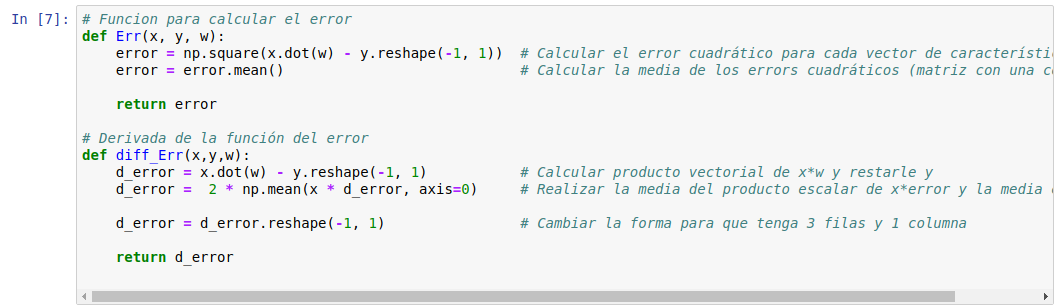
\includegraphics[scale=0.4]{img/func_error.png}
\caption{Función de error y derivada de ésta para el gradiente.}
\end{figure}

\begin{figure}[H]
\centering
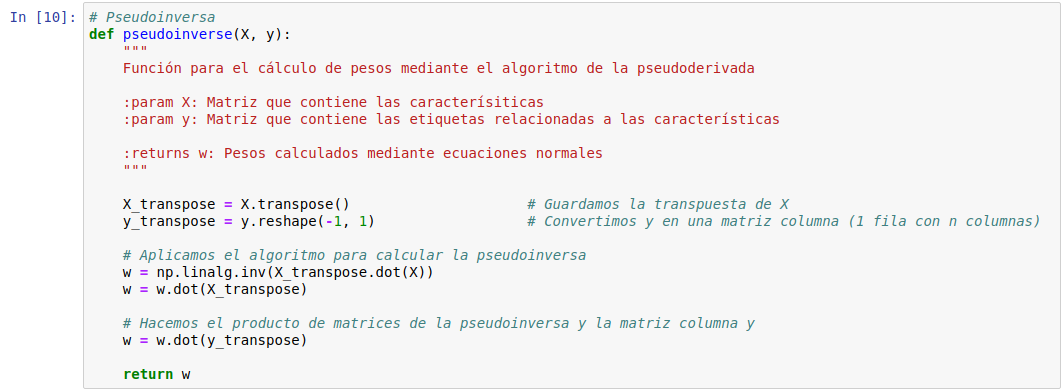
\includegraphics[scale=0.4]{img/pseudoinverse.png}
\caption{Implementación del algoritmo de la pseudoinversa.}
\end{figure}

\begin{figure}[H]
\centering
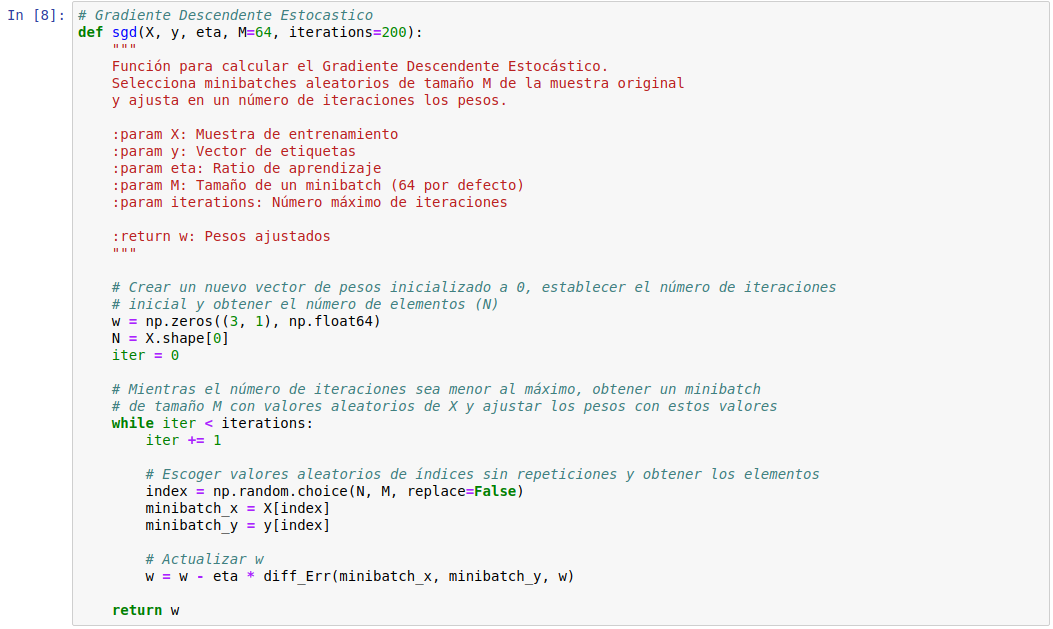
\includegraphics[scale=0.4]{img/sgd.png}
\caption{Implementación del Gradiente Descendente Estocástico.}
\end{figure}

Para realizar los ajustes utilizando el Gradiente Descendente Estocástico vamos a suponer una serie de cosas, ya que no
se especifican en el enunciado del problema:

\begin{itemize}[label=\textbullet]
	\item Como no se especifica cuántas iteraciones tiene que dar el algoritmo, vamos a suponer que, por defecto, da
	\textbf{200 iteraciones}.
	\item Como tampoco se especifica que $\eta$ utilizar, vamos a utilizar $\eta = 0.05$, ya que en combinación con el
	número de iteraciones, ofrece un buen resultado. También se ha probado con un $\eta = 0.01$ y se han conseguido
	resultados muy similares, pero con la contra de tener que realizar un mayor número de iteraciones.
	\item Como no se especifica ningún criterio para crear los \textit{batches}, vamos a escoger en cada iteración una
	parte aleatoria de la muestra de tamaño $M$, siendo $M = 64$ por defecto (y también el valor utilizado).
	\item Como tampoco se especifica un valor inicial para $w$, vamos a suponer que $w = \lbrace 0, 0, 0 \rbrace$.
\end{itemize}

Una vez dicho esto, vamos a ver los resultados de cada ajuste, comenzando con el Gradiente Descendente Estocástico:

\begin{figure}[H]
\centering
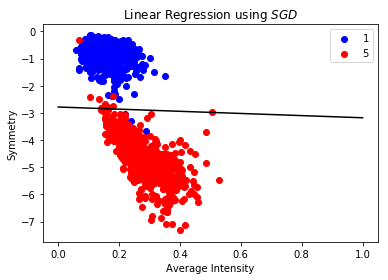
\includegraphics[scale=0.8]{img/sgd_regression.png}
\caption{Gráfica del ajuste de regresión mediante SGD.}
\end{figure}

\begin{figure}[H]
\centering
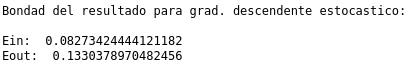
\includegraphics[scale=0.6]{img/sgd_regression_error.png}
\end{figure}

Como se puede comprobar, con los datos especificados anteriormente ($\eta = 0.05$, 200 iteraciones y $M = 64$) se obtiene
un ajuste muy bueno, si bien es cierto que van a haber algunos datos que no sean clasificados correctamente, ya que los
datos no son linealmente independientes del todo (se puede ver claramente que hay algunos datos cuyos valores no se
corresponden con la clase que supuestamente les toca).\\

Para poder pintar la recta, se ha pintado en el rango $[0, 1]$ (eje $X$) según los valores de $w$. Para ello, se ha
resuleto la ecuación $y = w_0 + w_1 x_1 + w_2 x_2$, donde $y$ es la clase obtenida, $x_1$ el valor en el eje $X$ y $x_2$ el
valor en el eje $Y$. En este caso se quería obtener el valor de $x_2$, ya que se han supuesto los casos en los que $x_1 = 0$
(extremo inferior del intervalo en el que se quiere pintar la recta) y $x_1 = 1$ (extremo superior del intervalo en el que se
quiere pintar la recta). Suponiento que $y = 0$ en ambos casos, se ha obtenido lo siguiente:

\[x_1 = 0, \: x_2 = \frac{-w_0}{w_2} \]
\[x_1 = 1, \: x_2 = \frac{-w_0 - w_1}{w_2} \]

Por tanto, los valores en el eje $Y$ tendrán en los extremos $[0, 1]$ los valores $[\frac{-w_0}{w_2}, \frac{-w_0 - w_1}{w_2}]$,
interpolando el resto de valores para poder formar la recta. Este mismo proceso se ha seguido para la pseudoinversa.\\

A continuación, vamos a observar los resultados del ajuste de regresión mediante la pseudoinversa:

\begin{figure}[H]
\centering
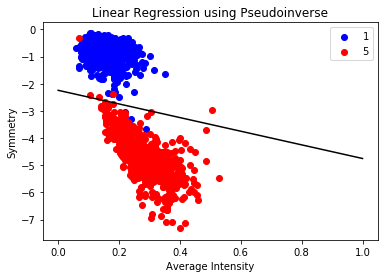
\includegraphics[scale=0.8]{img/pinv_regression.png}
\caption{Gráfica del ajuste de regresión mediante el algoritmo de la pseudoinversa.}
\end{figure}

\begin{figure}[H]
\centering
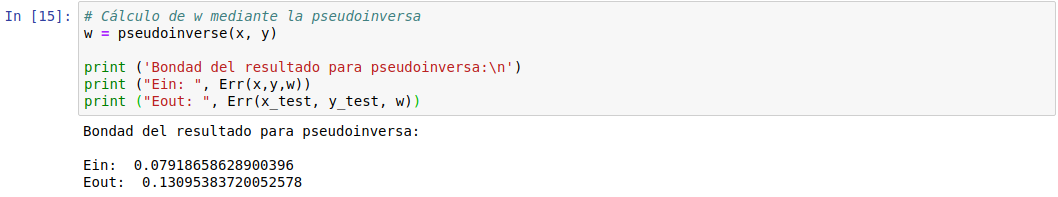
\includegraphics[scale=0.4]{img/pinv_error.png}
\caption{Resultados de los errores obtenidos con el ajuste de regresión para $E_{in}$ y $E_{out}$.}
\end{figure}

Como se puede ver, existen unas pequeñas diferencias. En este caso, la recta obtenida tiene un poco más de pendiente, y permite
obtener un error un poco menor en $E_{in}$, conservando sin embargo un error similar en $E_{out}$.\\

Ambas técnicas permiten obtener buenos resultados. Sin embargo, en este caso, la pseudoinversa permite obtener unos resultados
algo mejores, ya que intenta calcular los valores de $w$ resolviendo un sistema de ecuaciones, mientras que en el caso del
Gradiente Descendente Estocástico se intentan ajustar los valores de $w$ de forma iterativa y, al seleccionar elementos
aleatorios de la muestra, no se asegura que se realice un ajuste con todos los datos, lo cuál puede hacer que sea necesario
dar más iteraciones.

\subsection*{Apartado 2}
\noindent En este apartado exploramos como se transforman los errores $E_{in}$ y $E_{out}$ cuando aumentamos la complejidad
del modelo lineal usado. Ahora hacemos uso de la función $simula\_unif (N, 2, size)$ que nos devuelve $N$ coordenadas 2D de
puntos uniformemente muestreados dentro del cuadrado definido por $[-size, size] \times [-size, size]$

\begin{itemize}
	\item EXPERIMENTO
	\begin{enumerate}[label=\alph*)]
		\item Generar una muestra de entrenamiento de $N = 1000$ puntos en el cuadrado $X = [-1, 1] \times [-1, 1]$.
		Pintar el mapa de puntos 2D. (ver función de ayuda)
	\end{enumerate}
	
	Para generar los datos, hemos utilizado esta función:
	
	\begin{figure}[H]
	\centering
	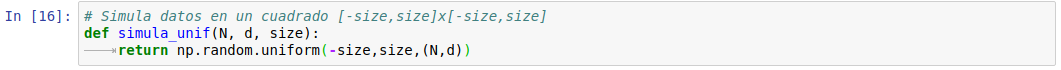
\includegraphics[scale=0.4]{img/simula_unif.png}
	\end{figure}
	
	Al generar los 1000 puntos, hemos obtenido el siguiente gráfico:
	
	\begin{figure}[H]
	\centering
	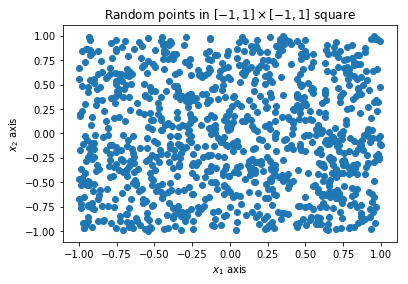
\includegraphics[scale=0.6]{img/random_points.png}
	\end{figure}
	
	\begin{enumerate}[resume, label=\alph*)]
		\item Consideremos la función $f(x_1, x_2) = \sign((x_1 - 0.2)^2 + x_2^2 - 0.6)$ que usaremos para asignar una
		etiqueta a cada punto de la muestra anterior. Introducimos ruido sobre las etiquetas cambiando aleatoriamente
		el signo de un 10\% de las mismas. Pintar el mapa de etiquetas obtenido.
	\end{enumerate}
	
	La implementación de la función es la siguiente:
	
	\begin{figure}[H]
	\centering
	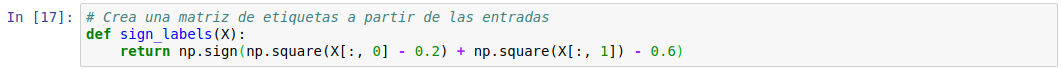
\includegraphics[scale=0.4]{img/sign_func.png}
	\end{figure}
	
	Al generar el signo para los puntos, se ha obtenido el siguiente gráfico:
	
	\begin{figure}[H]
	\centering
	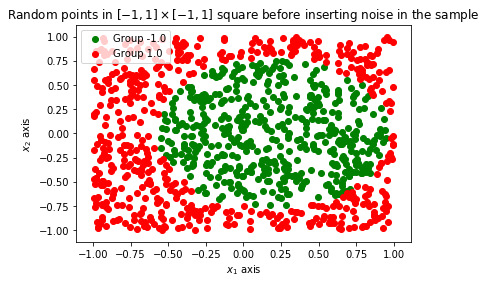
\includegraphics[scale=0.6]{img/sign_points.png}
	\end{figure}
	
	La función para insertar ruido es la siguiene:
	
	\begin{figure}[H]
	\centering
	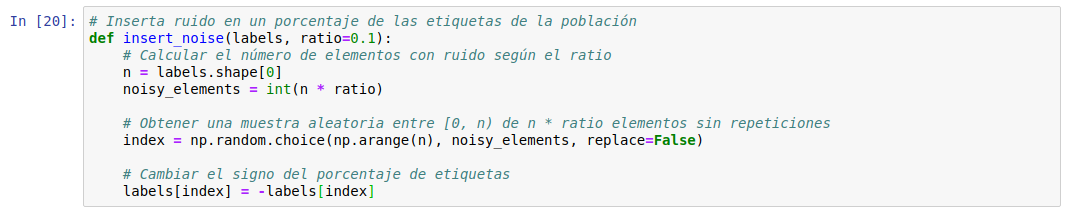
\includegraphics[scale=0.4]{img/noise_func.png}
	\end{figure}
	
	Tras insertar ruido, se ha obtenido el siguiente gráfico:
	
	\begin{figure}[H]
	\centering
	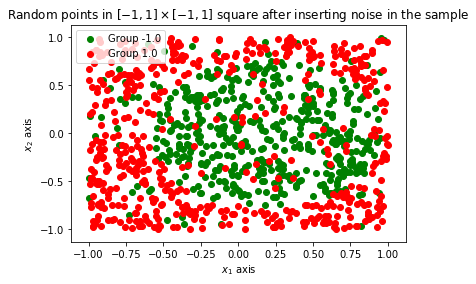
\includegraphics[scale=0.6]{img/random_noise.png}
	\end{figure}
	
	\begin{enumerate}[resume, label=\alph*)]
		\item Usando como vector de características $(1, x_1, x_2)$ ajustar un modelo de regresión lineal al conjunto de
		datos generado y estimar los pesos $w$. Estimar el error de ajuste $E_{in}$ usando Gradiente Descendente Estocástico
		(SGD).
	\end{enumerate}
	
	Al realizar el ajuste de regresión con el Gradiente Descendente Estocástico, hemos obtenido lo siguiente:
	
	\begin{figure}[H]
	\centering
	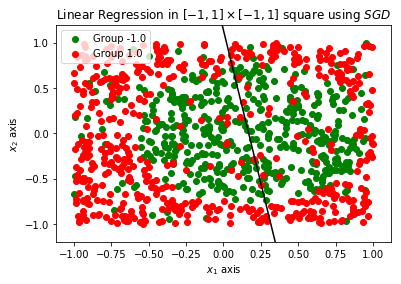
\includegraphics[scale=0.6]{img/random_regression.png}
	\caption{Gráfico del ajuste por regresión.}
	\end{figure}
	
	\begin{figure}[H]
	\centering
	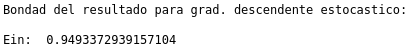
\includegraphics[scale=0.6]{img/random_error.png}
	\caption{Error para $E_{in}$.}
	\end{figure}
	
	Para dibujar la recta, se ha resuelto la misma ecuación que en el ejercicio anterior, solo que esta vez en el rango
	$[-1, 1]$, y se han obtenido los siguientes valores:
	
	\[x_1 = -1, \: x_2 = \frac{-w_0 + w_1}{w_2}\]
	\[x_1 = 1, \: x_2 = \frac{-w_0 - w_1}{w_2}\]
	
	\begin{enumerate}[resume, label=\alph*)]
		\item Ejecutar todo el experimento definido por (a)-(c) 1000 veces (generamos 1000 muestras diferentes) y
		\begin{itemize}
			\item Calcular el valor medio de los errores $E_{in}$ de las 1000 muestras.
			\item Generar 1000 puntos nuevos por cada iteración y calcular con ellos el valor de $E_{out}$ en dicha iteración.
			Calcular el valor medio de $E_{out}$ en todas las iteraciones.
		\end{itemize}
	\end{enumerate}
	
	Para el experimento repetido 1000 veces, se han obtenido los siguientes resultados:
	
	\begin{figure}[H]
	\centering
	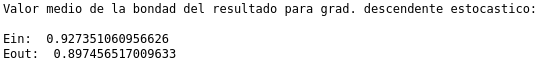
\includegraphics[scale=0.6]{img/random_1000_error.png}
	\end{figure}
	
	\begin{enumerate}[resume, label=\alph*)]
		\item Valore que tan bueno considera que es el ajuste con este modelo lineal a la vista de los valores medios
		obtenidos de $E_{in}$ y $E_{out}$.
	\end{enumerate}
	
	Los dos valores de los errores son muy malos, ya que están próximos a 1. Esto se debe a que una parte de los datos está
	dentro de la otra, y los modelos lineales están muy limitados en este aspecto, ya que una recta no puede dividir
	perfectamente los datos por mucho que se intente. Habría que utilizar otras funciones, como por ejemplo las hiperbólicas
	para intentar obtener un mejor ajuste.\\
	
	En el caso de $E_{in}$, el error obtendo es mayor que el de $E_{out}$, ya que al haber introducido ruido en la muestra
	de entrenamiento, los datos no serán linealmente independientes, y por tanto va a fallar más que de costumbre. En
	$E_{out}$, como no se ha metido ruido en las etiquetas, los datos no estarán tan dispersos, pero igualmente, no se
	podrá obtener un ajuste bueno por los motivos comentados anteriormente.
\end{itemize}


\section{Bonus}

\subsection*{Apartado 1}
\noindent \textbf{Método de Newton}. Implementar el algoritmo de minimización de Newton y aplicarlo a la función $f(x, y)$
dada en el ejercicio 3. Desarrolle los mismos experimentos usando los mismos puntos de inicio.

\begin{itemize}
	\item Generar un gráfico de como desciende el valor de la función con las iteraciones.
	\item Extraer conclusiones sobre las conductas de los algoritmos comparando la curva de decrecimiento de la función
	calculada en el apartado anterior y la correspondiente obtenida con el gradiente descendente.
\end{itemize}

Antes de empezar, vamos a calcular analíticamente el valor de la \textit{Hessiana}. Para ello, necesitamos calcular antes
$\frac{\partial^2 f}{\partial x^2}$, $\frac{\partial^2 f}{\partial y^2}$ y $\frac{\partial^2 f}{\partial xy}$:

\begin{equation}
\frac{\partial^2 f}{\partial x^2} = \frac{\partial^2}{\partial x^2} \Big(x^2 + 2y^2 + 2\sin(2 \pi x)\sin(2 \pi y)\Big) =
2 - 8 \pi ^ 2 \sin(2 \pi x)\sin(2 \pi y)
\end{equation}

\begin{equation}
\frac{\partial^2 f}{\partial y^2} = \frac{\partial^2}{\partial y^2} \Big(x^2 + 2y^2 + 2\sin(2 \pi x)\sin(2 \pi y)\Big) =
4 - 8 \pi ^ 2 \sin(2 \pi x)\sin(2 \pi y)
\end{equation}

\begin{equation}
\frac{\partial^2 f}{\partial xy} = \frac{\partial^2}{\partial xy} \Big(x^2 + 2y^2 + 2\sin(2 \pi x)\sin(2 \pi y)\Big) =
8 \pi ^ 2 \cos(2 \pi x)\cos(2 \pi y)
\end{equation}

Con lo cuál, tenemos que:

\begin{equation}
H =
\left[
{
\begin{array}{ccc}
	\frac{\partial^2 f}{\partial x^2} & & \frac{\partial^2 f}{\partial xy} \\
	\\
	\frac{\partial^2 f}{\partial xy} & & \frac{\partial^2 f}{\partial y^2}
\end{array}
}
\right]
\end{equation}

\begin{equation}
H =
\left[
{
\begin{array}{ccc}
	2 - 8 \pi ^ 2 \sin(2 \pi x)\sin(2 \pi y) & & 8 \pi ^ 2 \cos(2 \pi x)\cos(2 \pi y) \\
	\\
	8 \pi ^ 2 \cos(2 \pi x)\cos(2 \pi y) & & 4 - 8 \pi ^ 2 \sin(2 \pi x)\sin(2 \pi y)
\end{array}
}
\right]
\end{equation}\\

La implementación del algoritmo es la siguiente:

\begin{figure}[H]
\centering
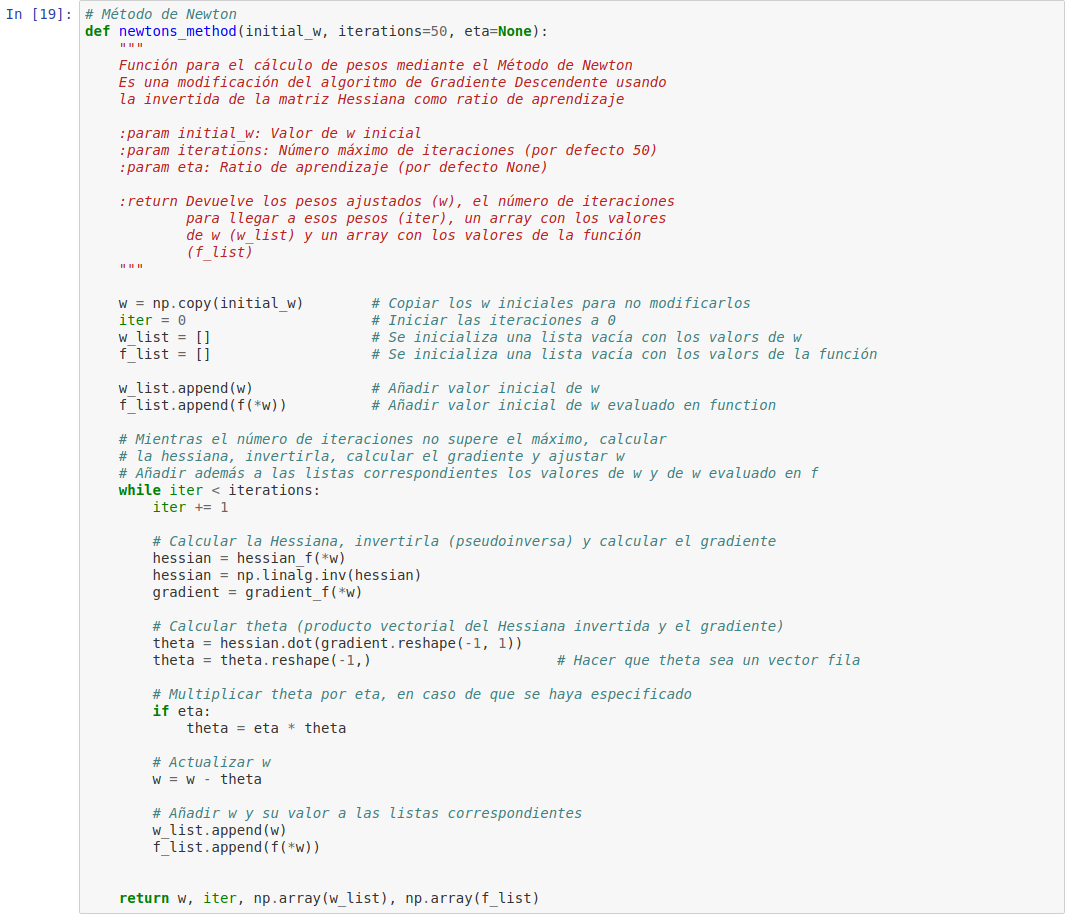
\includegraphics[scale=0.4]{img/nm_implementation.png}
\end{figure}

Una vez dicho esto, vamos a mostrar los resultados obtenidos:

\begin{figure}[H]
\centering
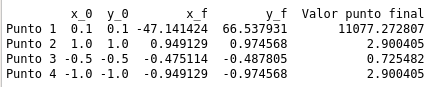
\includegraphics[scale=0.6]{img/nm_points.png}
\caption{Puntos obtenidos al aplicar el Método de Newton.}
\end{figure}

\begin{figure}[H]
\centering
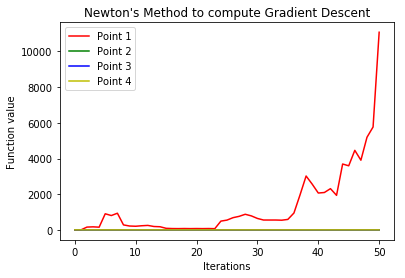
\includegraphics[scale=0.8]{img/nm_cmp.png}
\caption{Evolución de los valores de $f(x, y)$ con el Método de Newton.}
\end{figure}

\begin{figure}[H]
\centering
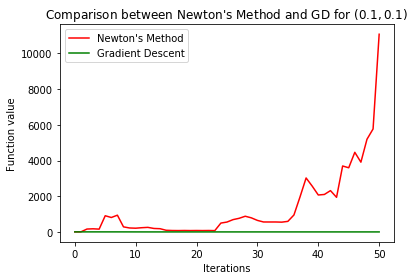
\includegraphics[scale=0.8]{img/nm_cmp1.png}
\caption{Minimización del punto $(0.1, 0.1)$ del GD comparada con el Método de Newton.}
\end{figure}

\begin{figure}[H]
\centering
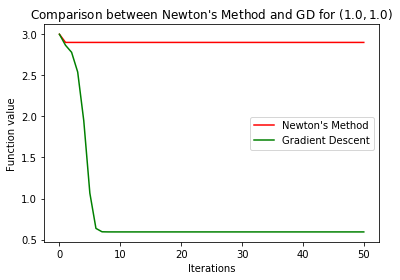
\includegraphics[scale=0.8]{img/nm_cmp2.png}
\caption{Minimización del punto $(1, 1)$ del GD comparada con el Método de Newton.}
\end{figure}

\begin{figure}[H]
\centering
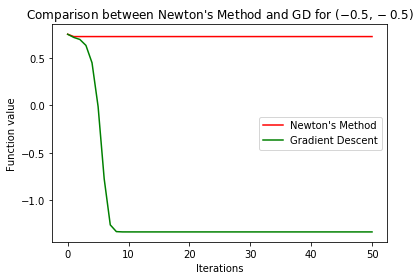
\includegraphics[scale=0.8]{img/nm_cmp3.png}
\caption{Minimización del punto $(-0.5, -0.5)$ del GD comparada con el Método de Newton.}
\end{figure}

\begin{figure}[H]
\centering
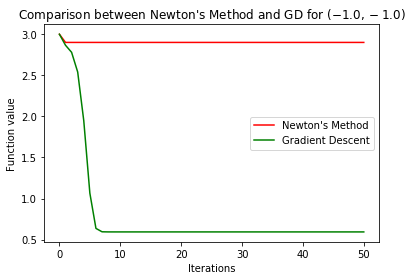
\includegraphics[scale=0.8]{img/nm_cmp4.png}
\caption{Minimización del punto $(-1, -1)$ del GD comparada con el Método de Newton.}
\end{figure}

Como se puede ver, las minimizacions no son muy buenas. En el primer caso es pésima ya que el valor de la función crece hasta
valores muy elevados, posiblemente debido a que el valor de la segunda derivada es muy elevado justo en el punto donde empieza,
con lo cuál sale disparada y empieza a crecer. En los otros casos, los valores de la función van decreciendo, pero a un ritmo
muy lento, con lo cuál tampoco se llega a un óptimo local, como en el primer caso.\\

Para intentar solucionar esto, vamos a meter un \textit{learning rate} $\eta = 0.01$ para evitar que en el primer caso el
Método de Newton haga que la función se salga disparada. Con esto obtenemos los siguientes resultados:\\

\begin{figure}[H]
\centering
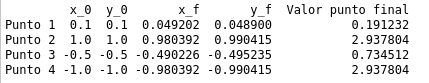
\includegraphics[scale=0.6]{img/nm_lr_points.png}
\caption{Puntos obtenidos al aplicar el Método de Newton con $\eta = 0.01$.}
\end{figure}

\begin{figure}[H]
\centering
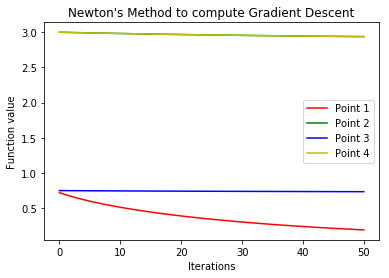
\includegraphics[scale=0.8]{img/nm_lr_cmp.png}
\caption{Evolución de los valores de $f(x, y)$ con el Método de Newton con $\eta  = 0.01$.}
\end{figure}

\begin{figure}[H]
\centering
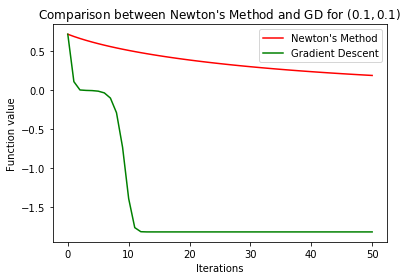
\includegraphics[scale=0.8]{img/nm_lr_cmp1.png}
\caption{Minimización del punto $(0.1, 0.1)$ del GD comparada con el Método de Newton con $\eta = 0.01$.}
\end{figure}

\begin{figure}[H]
\centering
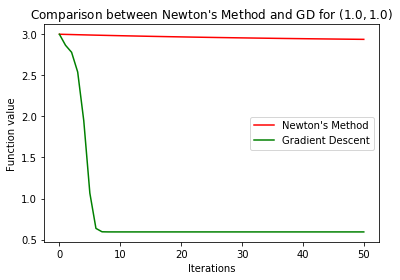
\includegraphics[scale=0.8]{img/nm_lr_cmp2.png}
\caption{Minimización del punto $(1, 1)$ del GD comparada con el Método de Newton con $\eta = 0.01$.}
\end{figure}

\begin{figure}[H]
\centering
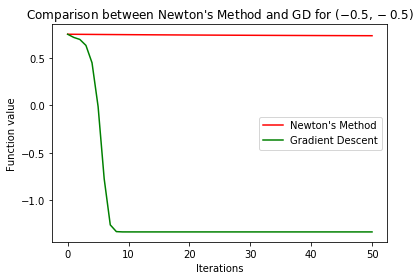
\includegraphics[scale=0.8]{img/nm_lr_cmp3.png}
\caption{Minimización del punto $(-0.5, -0.5)$ del GD comparada con el Método de Newton con $\eta = 0.01$.}
\end{figure}

\begin{figure}[H]
\centering
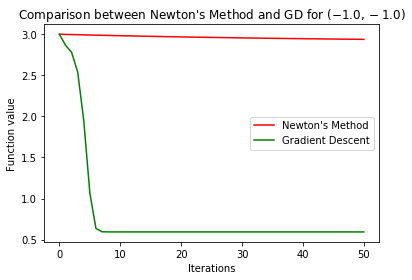
\includegraphics[scale=0.8]{img/nm_lr_cmp4.png}
\caption{Minimización del punto $(-1, -1)$ del GD comparada con el Método de Newton con $\eta = 0.01$.}
\end{figure}

Como se puede ver, al utilizar un $\eta = 0.01$, los valores son algo más normales. Para el primer punto se puede ver que
esta vez, en vez de salir disparado para arriba, los valores de la función se intentan acercar al óptimo local. En el resto
de casos, sin embargo, el ratio de descenso es aún peor que antes, con lo cuál los valores de la función descienden de una
forma mucho más lenta que antes. Además, como en la situación anterior, no se llega a converger en ningún momento. Ninguno
de los puntos llega a un óptimo local.\\

Las conclusiones que se pueden extraer del Método de Newton, en este caso, son las siguientes:
 
\begin{itemize}[label=\textbullet]
	\item La función no es la más adecuada, ya que no es completamente convexa. Tiene demasiados óptimos locales, y el punto
	de inicio condiciona mucho hacia dónde se dirige.
	\item Los puntos de inicio pueden no ser los más adecuados. En este caso, por ejemplo, el punto $(0.1, 0.1)$ tiene un valor
	de la segunda derivada muy próximo a 0. Por eso, al multiplicar el gradiente por la inversa de la Hessiana, se obtiene un
	valor muy elevado, lo cuál permite salir de la zona de mínimos y hace que los valores de la función obtenidos sean muy
	elevados y que solo vaya creciendo.
	\item El criterio de la segunda derivada no asegura que se consiga converger siempre a un óptimo local. En este caso,
	ninguno de los puntos consiguió llegar a un óptimo local, a pesar de que el Gradiente Descendente si que consiguió llegar,
	y que la segunda derivada ofrece una mayor velocidad de convergencia. Lo ideal sería combinar un \textit{learning rate}
	fijo con la segunda derivada cuando más se acerque al óptimo, para así acelerar la convergencia.
\end{itemize}

\end{document}

